% In this chapter, we have reviewed definite integrals, starting with the Fundamental Theorem of Calculus. We've looked at techniques for evaluating definite integrals algebraically, numerically, and graphically. We've reviewed Riemann sums, including the left, right, and midpoint approximations as well as the trapezoid rule. We have also looked at the average value of a function.

% This chapter also reviewed integrals based on parametrically defined functions, a BC Calculus topic.

\question
\[
\int_{-1}^{1}\left(x^{2}-x-1\right)\,dx=
\]
\begin{choices}
  \choice $\dfrac{2}{3}$
  \choice $0$
  \CorrectChoice $-\dfrac{4}{3}$
  \choice $-2$
  \choice $-1$
\end{choices}
\begin{solution}
The integral is equal to


\[
\left.\left(\dfrac{1}{3} x^{3}-\dfrac{1}{2} x^{2}-x\right)\right|_{-1} ^{1}=-\dfrac{7}{6}-\dfrac{1}{6}
\]


\end{solution}

\question
\[
\int_{1}^{2} \dfrac{3 x-1}{3 x}\,dx=
\]
\begin{choices}
  \choice $\dfrac{3}{4}$
  \CorrectChoice $1-\dfrac{1}{3} \ln 2$
  \choice $1-\ln 2$
  \choice $-\dfrac{1}{3} \ln 2$
  \choice $1$
\end{choices}
\begin{solution}
Rewrite as $\int_{1}^{2}\left(1-\dfrac{1}{3} \cdot \dfrac{1}{x}\right) d x$. This equals


\[
\left.\left(x-\dfrac{1}{3} \ln x\right)\right|_{1} ^{2}=2-\dfrac{1}{3} \ln 2-1
\]


\end{solution}

\question
\[
\int_{0}^{3} \dfrac{d t}{\sqrt{4-t}}=
\]
\begin{choices}
  \choice $1$
  \choice $-2$
  \choice $4$
  \choice $-1$
  \CorrectChoice $2$
\end{choices}
\begin{solution}
Rewrite as
\[
-\int_{0}^{3}(4-t)^{-1 / 2}(-1 d t)=-\left.2 \sqrt{4-t}\right|_{0} ^{3}=-2(1-2)
\]
\end{solution}



\newpage




\question
\[
\int_{-1}^{0} \sqrt{3 u+4}\,du=
\]
\begin{choices}
  \choice $2$
  \CorrectChoice $\dfrac{14}{9}$
  \choice $\dfrac{14}{3}$
  \choice $6$
  \choice $\dfrac{7}{2}$
\end{choices}
\begin{solution}
This integral equals


\[
\begin{aligned}
\dfrac{1}{3} \int_{-1}^{0}(3 u+4)^{1 / 2} \cdot 3 d u & =\left.\dfrac{1}{3} \cdot \dfrac{2}{3}(3 u+4)^{3 / 2}\right|_{-1} ^{0} \\
& =\dfrac{2}{9}\left(4^{3 / 2}-1^{3 / 2}\right)
\end{aligned}
\]


\end{solution}

\question
\[
\int_{2}^{3} \dfrac{d y}{2 y-3}=
\]
\begin{choices}
  \choice $\ln 3$
  \choice $\dfrac{1}{2} \ln \dfrac{3}{2}$
  \choice $\dfrac{16}{9}$
  \CorrectChoice $\ln \sqrt{3}$
  \choice $\sqrt{3}-1$
\end{choices}
\begin{solution}
$\quad \dfrac{1}{2} \int_{2}^{3} \dfrac{2 d y}{2 y-3}=\left.\dfrac{1}{2} \ln (2 y-3)\right|_{2} ^{3}=\dfrac{1}{2}(\ln 3-\ln 1)$
\end{solution}

\question
\[
\int_{0}^{\sqrt{3}} \dfrac{x}{\sqrt{4-x^{2}}}\,dx=
\]
\begin{choices}
  \CorrectChoice $1$
  \choice $\dfrac{\pi}{6}$
  \choice $\dfrac{\pi}{3}$
  \choice $-1$
  \choice $2$
\end{choices}
\begin{solution}
Rewrite as
\[
-\dfrac{1}{2} \int_{0}^{\sqrt{3}}\left(4-x^{2}\right)^{-1 / 2}(-2 x d x)=-\left.\dfrac{1}{2} \cdot 2 \sqrt{4-x^{2}}\right|_{0} ^{\sqrt{3}}=-(1-2)
\]
\end{solution}



\newpage





\question
\[
\int_{0}^{1}(2 t-1)^{3}\,dt=
\]
\begin{choices}
  \choice $\dfrac{1}{4}$
  \choice $6$
  \choice $\dfrac{1}{2}$
  \CorrectChoice $0$
  \choice $4$
\end{choices}
\begin{solution}
$\quad \dfrac{1}{2} \int_{0}^{1}(2 t-1)^{3}(2 d t)=\left.\dfrac{1}{2} \cdot \dfrac{(2 t-1)^{4}}{4}\right|_{0} ^{1}=\dfrac{1}{2}\left(\dfrac{(2 \cdot 1-1)^{4}}{4}-\dfrac{(2 \cdot 0-1)^{4}}{4}\right)$
\end{solution}

\question
\[
\int_{4}^{9} \dfrac{2+x}{2 \sqrt{x}}\,dx=
\]
\begin{choices}
  \CorrectChoice $\dfrac{25}{3}$
  \choice $\dfrac{41}{3}$
  \choice $\dfrac{100}{3}$
  \choice $\dfrac{5}{3}$
  \choice $\dfrac{1}{3}$
\end{choices}
\begin{solution}
Divide:
\[
\begin{aligned}
\int_{4}^{9}\left(x^{-1 / 2}+\dfrac{1}{2} x^{1 / 2}\right) d x & =\left.\left(2 x^{1 / 2}+\dfrac{1}{2} \cdot \dfrac{2}{3} x^{3 / 2}\right)\right|_{4} ^{9} \\
& =\left(2 \cdot 3+\dfrac{1}{3} \cdot 27\right)-\left(2 \cdot 2+\dfrac{1}{3} \cdot 8\right)
\end{aligned}
\]
\end{solution}




\newpage




\question
\[
\int_{-3}^{3} \dfrac{d x}{9+x^{2}}=
\]
\begin{choices}
  \choice $\dfrac{\pi}{2}$
  \choice $0$
  \CorrectChoice $\dfrac{\pi}{6}$
  \choice $-\dfrac{\pi}{2}$
  \choice $\dfrac{\pi}{3}$
\end{choices}
\begin{solution}
$\dfrac{1}{9} \int_{-3}^{3} \dfrac{d x}{1+\dfrac{x^{2}}{9}}=3 \cdot \dfrac{1}{9} \int_{-3}^{3} \dfrac{\dfrac{1}{3} d x}{1+\left(\dfrac{x}{3}\right)^{2}}=\left.\dfrac{1}{3} \tan ^{-1} \dfrac{x}{3}\right|_{-3} ^{3}=\dfrac{1}{3}\left(\dfrac{\pi}{4}-\left(-\dfrac{\pi}{4}\right)\right)$.
\end{solution}

\question
\[
\int_{0}^{1} e^{-x}\,dx=
\]
\begin{choices}
  \choice $\dfrac{1}{e}-1$
  \choice $1-e$
  \choice $-\dfrac{1}{e}$
  \CorrectChoice $1-\dfrac{1}{e}$
  \choice $\dfrac{1}{e}$
\end{choices}
\begin{solution}
You get $-\left.e^{-x}\right|_{0} ^{1}=-\left(e^{-1}-1\right)$.
\end{solution}

\question
\[
\int_{0}^{1} x e^{x^{2}}\,dx=
\]
\begin{choices}
  \choice $e-1$
  \CorrectChoice $\dfrac{1}{2}(e-1)$
  \choice $2(e-1)$
  \choice $\dfrac{e}{2}$
  \choice $\dfrac{e}{2}-1$
\end{choices}
\begin{solution}
$\dfrac{1}{2} \int_{0}^{1} e^{x^{2}}(2 x d x)=\left.\dfrac{1}{2} e^{x^{2}}\right|_{0} ^{1}=\dfrac{1}{2}(e-1)$.
\end{solution}




\newpage




\question
\[
\int_{0}^{\pi / 4} \sin 2 \theta\,d\theta=
\]
\begin{choices}
  \choice $2$
  \CorrectChoice $\dfrac{1}{2}$
  \choice $-1$
  \choice $-\dfrac{1}{2}$
  \choice $-2$
\end{choices}
\begin{solution}
Evaluate $-\left.\dfrac{1}{2} \cos 2 \theta\right|_{0} ^{\pi / 4}$, which equals $-\dfrac{1}{2}(0-1)$.
\end{solution}

\question
\[
\int_{1}^{2} \dfrac{d z}{3-z}=
\]
\begin{choices}
  \choice $-\ln 2$
  \choice $\dfrac{3}{4}$
  \choice $2(\sqrt{2}-1)$
  \choice $\dfrac{1}{2} \ln 2$
  \CorrectChoice $\ln 2$
\end{choices}
\begin{solution}
$-\int_{1}^{2} \dfrac{-d x}{3-z}=-\left.\ln (3-z)\right|_{1} ^{2}=-(\ln 1-\ln 2)$.
\end{solution}

\question
If we let $x=2 \sin \theta$, then $\int_{1}^{2} \dfrac{\sqrt{4-x^{2}}}{x} d x$ is equivalent to
\begin{choices}
  \choice $2 \int_{0}^{2} \dfrac{\cos ^{2} \theta}{\sin \theta}\,d\theta$
  \choice $\int_{\pi / 6}^{\pi / 2} \dfrac{\cos \theta}{\sin \theta}\,d\theta$
  \CorrectChoice $2 \int_{\pi / 6}^{\pi / 2} \dfrac{\cos ^{2} \theta}{\sin \theta}\,d\theta$
  \choice $\int_{1}^{2} \dfrac{\cos \theta}{\sin \theta}\,d\theta$
  \choice none of these
\end{choices}
\begin{solution}
If $x=2 \sin \theta, \sqrt{4-x^{2}}=2 \cos \theta, d x=2 \cos \theta\,d\theta$. When $x=1, \theta=\dfrac{\pi}{6}$; when $x=2, \theta=\dfrac{\pi}{2}$. The integral is equivalent to $\int_{\pi / 6}^{\pi / 2} \dfrac{(2 \cos \theta)(2 \cos \theta)\,d\theta}{2 \sin \theta}$.
\end{solution}




\newpage




\question
\[
\int_{0}^{\pi} \cos ^{2} \theta \sin \theta\,d\theta=
\]
\begin{choices}
  \choice $-\dfrac{2}{3}$
  \choice $\dfrac{1}{3}$
  \choice $1$
  \CorrectChoice $\dfrac{2}{3}$
  \choice $0$
\end{choices}
\begin{solution}
Evaluate $-\int_{0}^{\pi} \cos ^{2} \theta(-\sin \theta\,d\theta)$. This equals $-\left.\dfrac{1}{3} \cos ^{3} \theta\right|_{0} ^{\pi}=-\dfrac{1}{3}(-1-1)$.
\end{solution}

\question
\[
\int_{1}^{e} \dfrac{\ln x}{x}\,dx=
\]
\begin{choices}
  \CorrectChoice $\dfrac{1}{2}$
  \choice $\dfrac{1}{2}\left(e^{2}-1\right)$
  \choice $0$
  \choice $1$
  \choice $e-1$
\end{choices}
\begin{solution}
$\quad \int_{1}^{e}(\ln x)\left(\dfrac{1}{x} d x\right)=\left.\dfrac{1}{2} \ln ^{2} x\right|_{1} ^{e}=\dfrac{1}{2}(1-0)$.
\end{solution}

\question
\[
\int_{0}^{1} x e^{x}\,dx=
\]
\begin{choices}
  \choice $-1$
  \choice $e+1$
  \CorrectChoice $1$
  \choice $e-1$
  \choice $\dfrac{1}{2}(e-1)$
\end{choices}
\begin{solution}
Use the Parts Formula with $u=x$ and $d v=e^{x} d x$. Then $d u=d x$ and $v=e^{x}$. The result is
\[
\left.\left(x e^{x}-\int e^{x} d x\right)\right|_{0} ^{1}=\left.\left(x e^{x}-e^{x}\right)\right|_{0} ^{1}=(e-e)-(0-1)
\]
\end{solution}




\newpage




\question
\[
\int_{0}^{\pi / 6} \dfrac{\cos \theta}{1+2 \sin \theta}\,d\theta=
\]
\begin{choices}
  \choice $\ln 2$
  \choice $\dfrac{3}{8}$
  \choice $-\dfrac{1}{2} \ln 2$
  \choice $\dfrac{3}{2}$
  \CorrectChoice $\ln \sqrt{2}$
\end{choices}
\begin{solution}
$\dfrac{1}{2} \int_{0}^{\pi / 6} \dfrac{2 \cos \theta\,d\theta}{1+2 \sin \theta}=\left.\dfrac{1}{2} \ln (1+2 \sin \theta)\right|_{0} ^{\pi / 6}$ and get $\dfrac{1}{2}(\ln (1+1)-\ln 1)$.
\end{solution}

\question\label{calc06:u-over-u2-minus-1}
\[
\int_{\sqrt{2}}^{2} \dfrac{u}{u^{2}-1}\,du=
\]
\begin{choices}
  \CorrectChoice $\ln \sqrt{3}$
  \choice $\dfrac{8}{9}$
  \choice $\ln \dfrac{3}{2}$
  \choice $\ln 3$
  \choice $1-\sqrt{3}$
\end{choices}
\begin{solution}
Evaluate the integral $\dfrac{1}{2} \int_{\sqrt{2}}^{2} \dfrac{2 u}{u^{2}-1} d u$. It equals
\[
\left.\dfrac{1}{2} \ln \left(u^{2}-1\right)\right|_{\sqrt{2}} ^{2} \quad \text { or } \quad \dfrac{1}{2}(\ln 3-\ln 1)
\]
\end{solution}




\newpage




\question
\[
\int_{\sqrt{2}}^{2} \dfrac{u\,du}{\left(u^{2}-1\right)^{2}}=
\]
\begin{choices}
  \choice $-\dfrac{1}{3}$
  \choice $-\dfrac{2}{3}$
  \choice $\dfrac{2}{3}$
  \choice $-1$
  \CorrectChoice $\dfrac{1}{3}$
\end{choices}
\begin{solution}
Evaluate $\dfrac{1}{2} \int_{\sqrt{2}}^{2}\left(u^{2}-1\right)^{-2} \cdot 2 u d u$ and get


\[
-\left.\dfrac{1}{2\left(u^{2}-1\right)}\right|_{\sqrt{2}} ^{2} \quad \text { or } \quad-\dfrac{1}{2}\left(\dfrac{1}{3}-\dfrac{1}{1}\right)
\]

Compare with Question~\ref{calc06:u-over-u2-minus-1}.
\end{solution}

\question
\[
\int_{0}^{\pi / 4} \cos ^{2} \theta\,d\theta=
\]
\begin{choices}
  \choice $\dfrac{1}{2}$
  \choice $\dfrac{\pi}{8}$
  \CorrectChoice $\dfrac{\pi}{8}+\dfrac{1}{4}$
  \choice $\dfrac{\pi}{8}+\dfrac{1}{2}$
  \choice $\dfrac{\pi}{8}-\dfrac{1}{4}$
\end{choices}
\begin{solution}
(C) Use this identity: $\cos ^{2} \theta=\dfrac{1}{2}(1+\cos 2 \theta)$. Then
\[
\dfrac{1}{2} \int_{0}^{\pi / 4}(1+\cos 2 \theta)\,d\theta=\left.\dfrac{1}{2}\left(\theta+\dfrac{1}{2} \sin 2 \theta\right)\right|_{0} ^{\pi / 4}=\dfrac{1}{2}\left(\left(\dfrac{\pi}{4}+\dfrac{1}{2}\right)-0\right)
\]
\end{solution}




\newpage




\question
\[
\int_{\pi / 12}^{\pi / 4} \dfrac{\cos 2 x\,dx}{\sin ^{2} 2 x}=
\]
\begin{choices}
  \choice $-\dfrac{1}{4}$
  \choice $1$
  \CorrectChoice $\dfrac{1}{2}$
  \choice $-\dfrac{1}{2}$
  \choice $-1$
\end{choices}
\begin{solution}
Rewrite:
\[
\begin{aligned}
\dfrac{1}{2} \int_{\pi / 12}^{\pi / 4} \sin ^{-2} 2 x \cos 2 x(2 d x) & =-\left.\dfrac{1}{2} \cdot \dfrac{1}{\sin 2 x}\right|_{\pi / 12} ^{\pi / 4} \\
& =-\dfrac{1}{2}\left(\dfrac{1}{1}-\dfrac{1}{1 / 2}\right)
\end{aligned}
\]
\end{solution}

\question
\[
\int_{0}^{1} \dfrac{e^{-x}+1}{e^{-x}}\,dx=
\]
\begin{choices}
  \CorrectChoice $e$
  \choice $2+e$
  \choice $\dfrac{1}{e}$
  \choice $1+e$
  \choice $e-1$
\end{choices}
\begin{solution}
The integral is equivalent to
\[
\int_{0}^{1}\left(1+e^{x}\right) d x=\left.\left(x+e^{x}\right)\right|_{0} ^{1}=(1+e)-1
\]
\end{solution}




\newpage




\question
\[
\int_{0}^{1} \dfrac{e^{x}}{e^{x}+1}\,dx=
\]
\begin{choices}
  \choice $\ln 2$
  \choice $e$
  \choice $1+e$
  \choice $-\ln 2$
  \CorrectChoice $\ln \dfrac{e+1}{2}$
\end{choices}
\begin{solution}
Evaluate $\left.\ln \left(e^{x}+1\right)\right|_{0} ^{1}$, getting $\ln (e+1)-\ln 2$.
\end{solution}





\question
If we let $x=\tan \theta$, then $\int_{1}^{\sqrt{3}} \sqrt{1+x^{2}} d x$ is equivalent to
\begin{choices}
  \choice $\int_{\pi / 4}^{\pi / 3} \sec \theta\,d\theta$
  \choice $\int_{1}^{\sqrt{3}} \sec ^{3} \theta\,d\theta$
  \CorrectChoice $\int_{\pi / 4}^{\pi / 3} \sec ^{3} \theta\,d\theta$
  \choice $\int_{\pi / 4}^{\pi / 3} \sec ^{2} \theta \tan \theta\,d\theta$
  \choice $\int_{1}^{\sqrt{3}} \sec \theta\,d\theta$
\end{choices}
\begin{solution}
Note that $d x=\sec ^{2} \theta d \theta$ and that $\sqrt{1+\tan ^{2} \theta}=\sec \theta$. Be sure to express the limits as values of $\theta$ : $1=\tan \theta$ yields $\theta=\dfrac{\pi}{4} ; \sqrt{3}=\tan \theta$ yields $\theta=\dfrac{\pi}{3}$.
\end{solution}

\question
If the substitution $u=\sqrt{x+1}$ is used, then $\int_{0}^{3} \dfrac{d x}{x \sqrt{x+1}}$ is equivalent to
\begin{choices}
  \choice $\int_{1}^{2} \dfrac{d u}{u^{2}-1}$
  \CorrectChoice $\int_{1}^{2} \dfrac{2 d u}{u^{2}-1}$
  \choice $2 \int_{0}^{3} \dfrac{d u}{(u-1)(u+1)}$
  \choice $2 \int_{1}^{2} \dfrac{d u}{u\left(u^{2}-1\right)}$
  \choice $2 \int_{0}^{3} \dfrac{d u}{u(u-1)}$
\end{choices}
\begin{solution}
If $u=\sqrt{x+1}$, then $u^{2}=x+1$, and $2 u d u=d x$. When you substitute for the limits, you get $2 \int_{1}^{2} \dfrac{u d u}{u\left(u^{2}-1\right)}$. Since $u \neq 0$ on its interval of integration, you may divide numerator and denominator by it.
\end{solution}




\newpage




\question
Using $M(3)$, we find that the approximate area of the shaded region below is
\begin{center}
  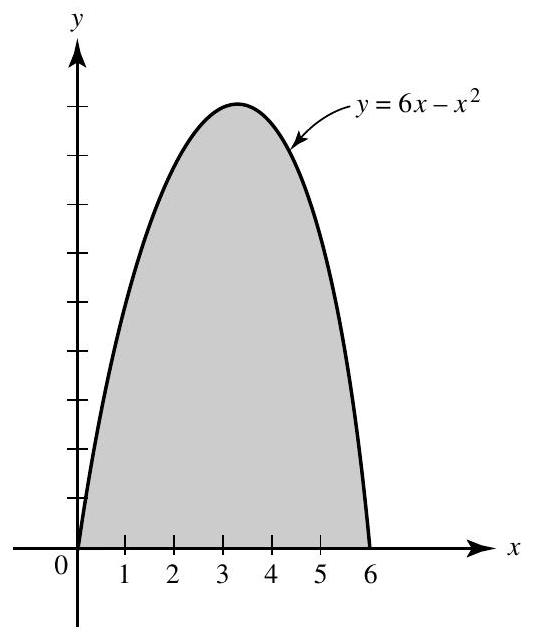
\includegraphics[width=0.45\linewidth]{calculus/images/2938c7af-d3ff-4e8a-bcfe-0da8db8771ce-04_637_535_1753_1087.jpg}
\end{center}
\begin{choices}
  \choice $9$
  \choice $19$
  \choice $36$
  \CorrectChoice $38$
  \choice $54$
\end{choices}
\begin{solution}
On $[0,6]$ with $n=3, \Delta x=2$. Heights of rectangles at $x=1,3$, and 5 are 5 , 9 , and 5, respectively; $M(3)=(5+9+5)(2)$.
\end{solution}

\question
The graph of a continuous function $f$ passes through the points $(4,2),(6,6),(7,5)$, and $(10,8)$. Using trapezoids, we estimate that $\int_{4}^{10} f(x) d x \approx$
\begin{choices}
  \choice $25$
  \choice $30$
  \choice $32$
  \CorrectChoice $33$
  \choice $41$
\end{choices}
\begin{solution}
$\quad \int_{4}^{10} f(x) d x \approx\left(\dfrac{2+6}{2}\right) \cdot 2+\left(\dfrac{6+5}{2}\right) \cdot 1+\left(\dfrac{5+8}{2}\right) \cdot 3 \approx 33$
\end{solution}




\newpage




\question
The area of the shaded region in the figure is equal exactly to $\ln 3$. If we approximate $\ln 3$ using $L(2)$ and $R(2)$, which inequality follows?
\begin{center}
  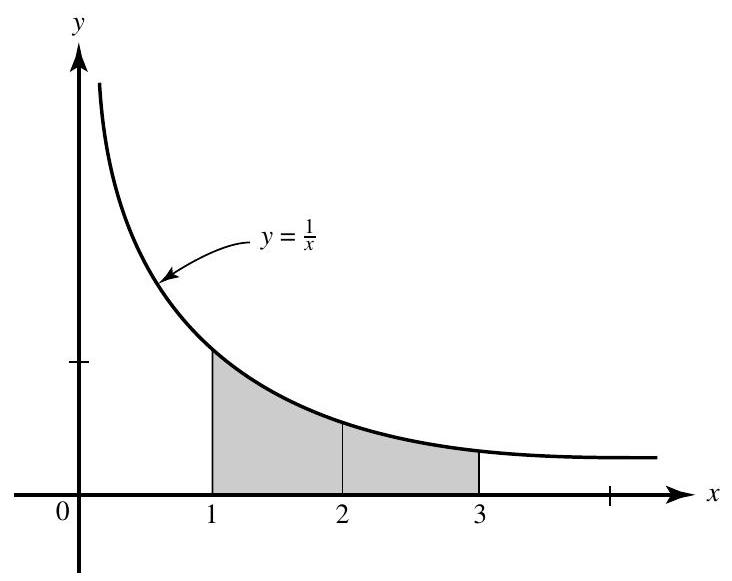
\includegraphics[width=0.7\linewidth]{calculus/images/2938c7af-d3ff-4e8a-bcfe-0da8db8771ce-05_581_732_419_616.jpg}
\end{center}
\begin{choices}
  \choice $\dfrac{1}{2}<\int_{1}^{2} \dfrac{1}{x} d x<1$
  \choice $\dfrac{1}{3}<\int_{1}^{3} \dfrac{1}{x} d x<2$
  \choice $\dfrac{1}{2}<\int_{0}^{2} \dfrac{1}{x} d x<2$
  \choice $\dfrac{1}{3}<\int_{2}^{3} \dfrac{1}{x} d x<\dfrac{1}{2}$
  \CorrectChoice $\dfrac{5}{6}<\int_{1}^{3} \dfrac{1}{x} d x<\dfrac{3}{2}$
\end{choices}
\begin{solution}
For $L(2)$ use the circumscribed rectangles:
\[
1 \cdot 1+\dfrac{1}{2} \cdot 1=\dfrac{3}{2}
\]
for $R(2)$ use the inscribed rectangles:
\[
\dfrac{1}{2} \cdot 1+\dfrac{1}{3} \cdot 1=\dfrac{5}{6}
\]
\end{solution}




\newpage




\question
Let $A=\int_{0}^{1} \cos x d x$. We estimate $A$ using the $L, R$, and $T$ approximations with $n=100$ subintervals. Which is true?
\begin{choices}
  \choice $L<A<T<R$
  \choice $L<T<A<R$
  \choice $R<A<T<L$
  \CorrectChoice $R<T<A<L$
  \choice The order cannot be determined.
\end{choices}
\begin{solution}
On $[0,1] f(x)=\cos x$ is decreasing, so $R<L$. Furthermore, $f$ is concave downward, so $T<A$.
\end{solution}

\question
\[
\int_{-1}^{3}|x|\,dx=
\]
\begin{choices}
  \choice $\dfrac{7}{2}$
  \choice $4$
  \choice $\dfrac{9}{2}$
  \CorrectChoice $5$
  \choice $\dfrac{11}{2}$
\end{choices}
\begin{solution}
Rewrite the integral to evaluate it, using the fact that $x$ changes sign at 0.
The result is
\[
\int_{-1}^{0}(-x) d x+\int_{0}^{3} x d x=-\left.\dfrac{x^{2}}{2}\right|_{-1} ^{0}+\left.\dfrac{x^{2}}{2}\right|_{0} ^{3}
\]
Draw a sketch of $y=|x|$, and verify that the area over $-1 \leqq x \leqq 3$ equals 5.
\end{solution}




\newpage




\question
\[
\int_{-3}^{2}|x+1|\,dx=
\]
\begin{choices}
  \choice $\dfrac{5}{2}$
  \choice $\dfrac{7}{2}$
  \choice $5$
  \choice $\dfrac{11}{2}$
  \CorrectChoice $\dfrac{13}{2}$
\end{choices}
\begin{solution}
(E) Since $x+1$ changes sign at $x=-1,|x+1|=-(x+1)$ if $x<-1$ but equals $x+1$ if $x \geqq-1$. The given integral is therefore equivalent to

\[
\begin{aligned}
\int_{-3}^{-1}-(x+1) d x+\int_{-1}^{2}(x+1) d x & =-\left.\dfrac{(x+1)^{2}}{2}\right|_{-3} ^{-1}+\left.\dfrac{(x+1)^{2}}{2}\right|_{-1} ^{2} \\
& =-\dfrac{1}{2}(0-4)+\dfrac{1}{2}(9-0)
\end{aligned}
\]

Draw a sketch of $y=|x+1|$, and verify that the area over $-3 \leqq x \leqq 2$ is $\dfrac{13}{2}$.
\end{solution}

\question
The average value of $y=\sqrt{64-x^{2}}$ on its domain is
\begin{choices}
  \choice $2$
  \choice $4$
  \CorrectChoice $2 \pi$
  \choice $4 \pi$
  \choice none of these
\end{choices}
\begin{solution}
(C) Because $y=\sqrt{64-x^{2}}$ is a semicircle of radius 8 , its area is $32 \pi$. The domain is $[-8,8]$, or 16 units wide. Hence the average height of the function is $\dfrac{32 \pi}{16}$.
\end{solution}




\newpage




\question
The average value of $\cos x$ over the interval $\dfrac{\pi}{3} \leqq x \leqq \dfrac{\pi}{2}$ is
\begin{choices}
  \choice $\dfrac{3}{\pi}$
  \choice $\dfrac{1}{2}$
  \CorrectChoice $\dfrac{3(2-\sqrt{3})}{\pi}$
  \choice $\dfrac{3}{2 \pi}$
  \choice $\dfrac{2}{3 \pi}$
\end{choices}
\begin{solution}
(C) The average value is equal to $\dfrac{1}{\pi / 2-\pi / 3} \int_{\pi / 3}^{\pi / 2} \cos x d x$.
\end{solution}

\question
The average value of $\csc ^{2} x$ over the interval from $x=\dfrac{\pi}{6}$ to $x=\dfrac{\pi}{4}$ is
\begin{choices}
  \choice $\dfrac{3 \sqrt{3}}{\pi}$
  \choice $\dfrac{\sqrt{3}}{\pi}$
  \CorrectChoice $\dfrac{12}{\pi}(\sqrt{3}-1)$
  \choice $3 \sqrt{3}$
  \choice $3(\sqrt{3}-1)$
\end{choices}
\begin{solution}
(C) The average value is equal to $\dfrac{1}{\pi / 4-\pi / 6} \int_{\pi / 6}^{\pi / 4} \csc ^{2} x d x$.
\end{solution}




\newpage




\question
Find the average value of function $f$, as shown in the graph below, on the interval [0,5].
\begin{center}
  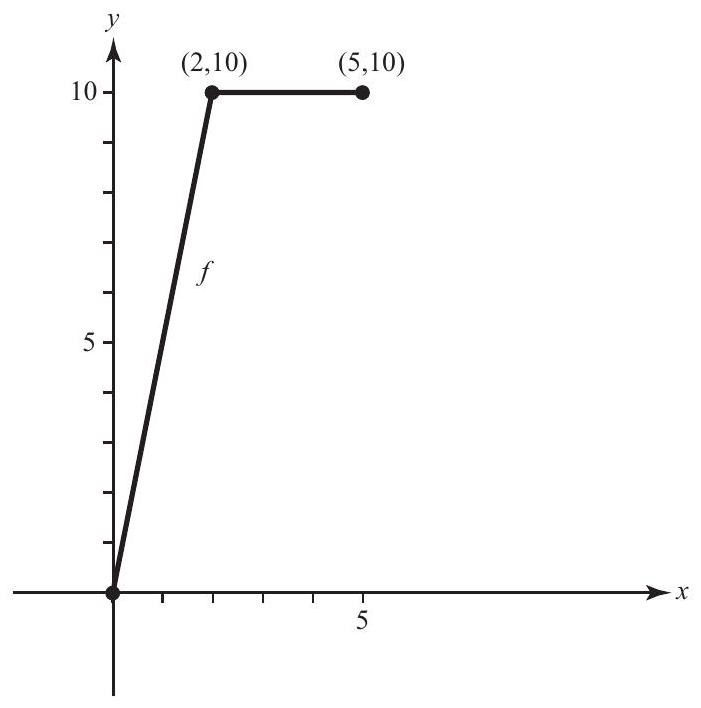
\includegraphics[width=0.45\linewidth]{calculus/images/2938c7af-d3ff-4e8a-bcfe-0da8db8771ce-06_708_701_1215_1002.jpg}
\end{center}
\begin{choices}
  \choice $2$
  \choice $4$
  \choice $5$
  \choice $7$
  \CorrectChoice $8$
\end{choices}
\begin{solution}
(E) The average value is $\dfrac{1}{5-0} \int_{0}^{5} f(x) d x$, where the integral represents the area of a trapezoid. That area is $\dfrac{1}{2}(5+3) \cdot 10=40$ making the average value $\dfrac{1}{5}(40)$.
\end{solution}

\question
The integral $\int_{-4}^{4} \sqrt{16-x^{2}} d x$ gives the area of
\begin{choices}
  \choice a circle of radius 4
  \CorrectChoice a semicircle of radius 4
  \choice a quadrant of a circle of radius 4
  \choice an ellipse whose semimajor axis is 4
  \choice none of these
\end{choices}
\begin{solution}
(B) Since $x^{2}+y^{2}=16$ is a circle, the given integral equals the area of a semicircle of radius 4 .
\end{solution}



\newpage




\question
\[
\int_{0}^{\pi / 4} \sqrt{1-\cos 2 \alpha} d \alpha=
\]
\begin{choices}
  \choice $0.25$
  \CorrectChoice $0.414$
  \choice $1.000$
  \choice $1.414$
  \choice $2.000$
\end{choices}
\begin{solution}
(B) Use a graphing calculator.
\end{solution}

\question
If $f(x)$ is continuous on the interval $a \leq x \leq b$ and $a<c<b$, then $\int_{c}^{b} f(x) d x$ is equal to
\begin{choices}
  \choice $\int_{a}^{c} f(x) d x+\int_{c}^{b} f(x) d x$
  \choice $\int_{a}^{c} f(x) d x-\int_{a}^{b} f(x) d x$
  \choice $\int_{c}^{a} f(x) d x+\int_{b}^{a} f(x) d x$
  \CorrectChoice $\int_{a}^{b} f(x) d x-\int_{a}^{c} f(x) d x$
  \choice $\int_{a}^{c} f(x) d x-\int_{b}^{c} f(x) d x$
\end{choices}
\begin{solution}
(D) Note that the integral from $a$ to $b$ is the sum of the two integrals from $a$ to $c$ and from $c$ to $b$.
\end{solution}

\question
If $f(x)$ is continuous on $a \leq x \leq b$, then
\begin{choices}
  \choice $\int_{a}^{b} f(x) d x=f(b)-f(a)$
  \CorrectChoice $\int_{a}^{b} f(x) d x=-\int_{b}^{a} f(x) d x$
  \choice $\int_{a}^{b} f(x) d x \geqq 0$
  \choice $\dfrac{d}{d x} \int_{a}^{x} f(t) d t=f^{\prime}(x)$
  \choice $\dfrac{d}{d x} \int_{a}^{x} f(t) d t=f(x)-f(a)$
\end{choices}
\begin{solution}
(B) In (A), we'd need to use the antiderivative of $f$ to evaluate the definite integral. In (C) if $f(x)<0$, the definite integral would be negative. In (D) and (E), the correct derivative of the definite integral would be $f(x)$.
\end{solution}




\newpage




\question
If $f(x)$ is continuous on the interval $a \leqq x \leqq b$, if this interval is partitioned into $n$ equal subintervals of length $\Delta x$, and if $x_{k}$ is a number in the $k$ th subinterval, then $\lim\limits_{n \to \infty} \sum_{1}^{n} f\left(x_{k}\right) \Delta x$ is equal to
\begin{choices}
  \choice $f(b)-f(a)$
  \choice $F(x)+C$, where $\dfrac{d F(x)}{d x}=f(x)$ and $C$ is an arbitrary constant
  \CorrectChoice $\int_{a}^{b} f(x) d x$
  \choice $F(b-a)$, where $\dfrac{d F(x)}{d x}=f(x)$
  \choice none of these
\end{choices}
\begin{solution}
(C) This is the definition of the definite integral given on page 249. As antiderivatives of $F^{\prime}$ and $G^{\prime}, F$ and $G$ may differ by a constant.
\end{solution}

\question
If $F^{\prime}(x)=G^{\prime}(x)$ for all $x$, then
\begin{choices}
  \CorrectChoice $\int_{a}^{b} F^{\prime}(x) d x=\int_{a}^{b} G^{\prime}(x) d x$
  \choice $\int F(x) d x=\int G(x) d x$
  \choice $\int_{a}^{b} F(x) d x=\int_{a}^{b} G(x) d x$
  \choice $\int F(x) d x=\int G(x) d x+C$
  \choice $F(x)=G(x)$ for all $x$.
\end{choices}
\begin{solution}
(A) Find examples of functions $F$ and $G$ that show that (B), (C), and (D) are false.
\end{solution}

\question
If $f(x)$ is continuous on the closed interval $[a, b]$, then there exists at least one number $c, a<c<b$, such that $\int_{a}^{b} f(x) d x$ is equal to
\begin{choices}
  \choice $\dfrac{f(c)}{b-a}$
  \choice $f^{\prime}(c)(b-a)$
  \CorrectChoice $f(c)(b-a)$
  \choice $\dfrac{f^{\prime}(c)}{b-a}$
  \choice $f(c)[f(b)-f(a)]$
\end{choices}
\begin{solution}
(C) This is the Mean Value Theorem for Integrals (page 250).
\end{solution}




\newpage




\question
If $f(x)$ is continuous on the closed interval $[a, b]$ and $k$ is a constant, then $\int_{a}^{b} k f(x) d x$ is equal to
\begin{choices}
  \choice $k(b-a)$
  \choice $k[f(b)-f(a)]$
  \choice $k F(b-a)$, where $\dfrac{d F(x)}{d x}=f(x)$
  \CorrectChoice $k \int_{a}^{b} f(x) d x$
  \choice $\left.\quad \dfrac{[k f(x)]^{2}}{2}\right]_{a}^{b}$
\end{choices}
\begin{solution}
(D) This is theorem (2) on page 250. Prove by counterexamples that (A), (B), (C), and (D) are false.
\end{solution}

\question
\[
\dfrac{d}{d t} \int_{0}^{t} \sqrt{x^{3}+1}\,dx=
\]
\begin{choices}
  \CorrectChoice $\sqrt{t^{3}+1}$
  \choice $\dfrac{\sqrt{t^{3}+1}}{3 t^{2}}$
  \choice $\dfrac{2}{3}\left(t^{3}+1\right)\left(\sqrt{t^{3}+1}-1\right)$
  \choice $3 x^{2} \sqrt{x^{3}+1}$
  \choice none of these
\end{choices}
\begin{solution}
(A) This is a restatement of the Fundamental Theorem. In theorem (1) on page 250, interchange $t$ and $x$.
\end{solution}

\question
If $F(u)=\int_{1}^{u}\left(2-x^{2}\right)^{3} d x$, then $F^{\prime}(u)$ is equal to
\begin{choices}
  \choice $-6 u\left(2-u^{2}\right)^{2}$
  \choice $\dfrac{\left(2-u^{2}\right)^{4}}{4}-\dfrac{1}{4}$
  \choice $\left(2-u^{2}\right)^{3}-1$
  \CorrectChoice $\left(2-u^{2}\right)^{3}$
  \choice $-2 u\left(2-u^{2}\right)^{3}$
\end{choices}
\begin{solution}
(D) Apply theorem (1) on page 250 , noting that
\[
F^{\prime}(u)=\dfrac{d}{d u} \int_{a}^{u} f(x) d x=f(u)
\]
\end{solution}




\newpage




\question
\[
\dfrac{d}{d x} \int_{\pi / 2}^{x^{2}} \sqrt{\sin t}\,dt=
\]
\begin{choices}
  \choice $\sqrt{\sin t^{2}}$
  \choice $2 x \sqrt{\sin x^{2}}-1$
  \choice $\dfrac{2}{3}\left(\sin ^{3 / 2} x^{2}-1\right)$
  \choice $\sqrt{\sin x^{2}}-1$
  \CorrectChoice $2 x \sqrt{\sin x^{2}}$.
\end{choices}
\begin{solution}
Let $y=\int_{\pi / 2}^{x^{2}} \sqrt{\sin t} d t$ and $u=x^{2}$; then


\[
y=\int_{\pi / 2}^{u} \sqrt{\sin t} d t
\]

By the Chain Rule, $\dfrac{d y}{d x}=\dfrac{d y}{d u} \cdot \dfrac{d u}{d x}=\sqrt{\sin u} \cdot 2 x$, where theorem (1) on page 250 is used to find $\dfrac{d y}{d u}$. Replace $u$ by $x^{2}$.
\end{solution}

\question
If $x=4 \cos \theta$ and $y=3 \sin \theta$, then $\int_{2}^{4} x y d x$ is equivalent to
\begin{choices}
  \choice $48 \int_{\pi / 3}^{0} \sin \theta \cos ^{2} \theta\,d\theta$
  \choice $48 \int_{2}^{4} \sin ^{2} \theta \cos \theta\,d\theta$
  \choice $36 \int_{2}^{4} \sin \theta \cos ^{2} \theta\,d\theta$
  \choice $-48 \int_{0}^{\pi / 3} \sin \theta \cos ^{2} \theta\,d\theta$
  \CorrectChoice $48 \int_{0}^{\pi / 3} \sin ^{2} \theta \cos \theta\,d\theta$
\end{choices}
\begin{solution}
(E) Since $d x=-4 \sin \theta\,d\theta$, you get the new integral $-48 \int_{\pi / 3}^{0} \sin ^{2} \theta \cos \theta\,d\theta$. Use theorem (4) on page 250 to get the correct answer.
\end{solution}

\question
A curve is defined by the parametric equations $y=2 a \cos ^{2} \theta$ and $x=2 a \tan \theta$, where $0 \leqq \theta \leqq \pi$. Then the definite integral $\pi \int_{0}^{2 a} y^{2} d x$ is equivalent to
\begin{choices}
  \choice $4 \pi a^{2} \int_{0}^{\pi / 4} \cos ^{4} \theta\,d\theta$
  \choice $8 \pi a^{3} \int_{\pi / 2}^{\pi} \cos ^{2} \theta\,d\theta$
  \CorrectChoice $8 \pi a^{3} \int_{0}^{\pi / 4} \cos ^{2} \theta\,d\theta$
  \choice $8 \pi a^{3} \int_{0}^{2 a} \cos ^{2} \theta\,d\theta$
  \choice $8 \pi a^{3} \int_{0}^{\pi / 4} \sin \theta \cos ^{2} \theta\,d\theta$
\end{choices}
\begin{solution}
(C) Since $d x=2 a \sec ^{2} \theta\,d\theta$, you get $8 \pi a^{3} \int_{0}^{\pi / 4} \cos ^{4} \theta \sec ^{2} \theta\,d\theta$. Use the fact that $$\cos ^{2} \theta \sec ^{2} \theta=1$$.
\end{solution}




\newpage




\question
A curve is given parametrically by $x=1-\cos t$ and $y=t-\sin t$, where $0 \leqq t \leqq \pi$. Then $\int_{0}^{3 / 2} y d x$ is equivalent to
\begin{choices}
  \choice $\int_{0}^{3 / 2} \sin t(t-\sin t) d t$
  \choice $\int_{2 \pi / 3}^{\pi} \sin t(t-\sin t) d t$
  \choice $\int_{0}^{2 \pi / 3}(t-\sin t) d t$
  \CorrectChoice $\int_{0}^{2 \pi / 3} \sin t(t-\sin t) d t$
  \choice $\int_{0}^{3 / 2}(t-\sin t) d t$
\end{choices}
\begin{solution}
(D) Use the facts that $d x=\sin t d t$, that $t=0$ when $x=0$, and that $t=\dfrac{2 \pi}{3}$ when $x=\dfrac{3}{2}$.
\end{solution}

\question
When $\int_{0}^{1} \sqrt{1+x^{2}} d x$ is estimated using $n=5$ subintervals of equal with, which is (are) true?

\statementbox{%
\begin{enumerate}
\renewcommand{\labelenumi}{\Roman{enumi}.}
\item $L(5)=\left(1+\sqrt{1+0.2^{2}}+\sqrt{1+0.4^{2}}+\sqrt{1+0.6^{2}}+\sqrt{1+0.8^{2}}\right)$
\item $M(5)=\left(\sqrt{1+0.1^{2}}+\sqrt{1+0.3^{2}}+\sqrt{1+0.5^{2}}+\sqrt{1+0.7^{2}}+\sqrt{1+0.9^{2}}\right) \cdot(0.2)$
\item $T(5)=\dfrac{0.2}{2}\left(1+2 \sqrt{1+0.2^{2}}+2 \sqrt{1+0.4^{2}}+2 \sqrt{1+0.6^{2}}+2 \sqrt{1+0.8^{2}}+\sqrt{2}\right)$
\end{enumerate}%
}
\begin{choices}
  \choice II only
  \choice III only
  \choice I and II only
  \choice I and III only
  \CorrectChoice II and III only
\end{choices}
\begin{solution}
(E) The expression for $L(5)$ does not multiply the heights of the rectangles by $\Delta x=0.2$.
\end{solution}

\question
Find the value of $x$ at which the function $y=x^{2}$ reaches its average value on the interval [0,10].
\begin{choices}
  \choice $4.642$
  \choice $5$
  \choice $5.313$
  \CorrectChoice $5.774$
  \choice $7.071$
\end{choices}
\begin{solution}
(D) The average value is $\dfrac{1}{10-0} \int_{0}^{10} x^{2} d x=\left.\dfrac{1}{10} \cdot \dfrac{x^{3}}{3}\right|_{0} ^{10}=\dfrac{100}{3}$. Solve $x^{2}=\dfrac{100}{3}$.
\end{solution}
